\documentclass{article}

% Target journal: Molecular Phylogenetics and Evolution
% Short communications of approximately 3000 words are also accepted. 
% These papers should contain no more than two figures, two tables, and thirty references. 
% A short abstract of fewer than 200 words is acceptable.

% Bibliography
\usepackage{natbib}
\bibpunct{(}{)}{;}{a}{}{;}

\usepackage[english]{babel}

% Use 'It was found that something is something (Name 1234)' style
\setcitestyle{authoryear,open={},close={}}

% Affiliations
\usepackage{authblk}
\title{The error in Bayesian phylogenetic reconstruction when speciation is not instantaneous}

\author[1]{Rich\`el J.C. Bilderbeek}
\author[1]{Rampal S. Etienne}
\affil[1]{Groningen Institute for Evolutionary Life Sciences, University of Groningen, Groningen, The Netherlands}

% Use double spacing
\usepackage{setspace}
\doublespacing

\usepackage{pgf}
\usepackage{hyperref}
\usepackage{verbatim}
  
% Adds numbered lines
\usepackage{lineno}
\linenumbers

\begin{document}

\maketitle

\begin{abstract}

  % From 'How to construct a Nature summary paragraph'

  % A short abstract of fewer than 200 words is acceptable.

  % One or two sentences providing a basic
  % introduction to the field,
  % comprehensible to a scientist in any discipline.
  The tools for reconstructing phylogenetic relationships between taxonomic 
  units (e.g. species) have become very advanced in the last three decades. 

  % Two to three sentences of
  % more detailed background, comprehensible to
  % scientists in related disciplines.
  Among the most popular tools are Bayesian approaches, 
  such as BEAST, MrBayes and RevBayes, 
  that use efficient tree sampling routines to create a posterior probability distribution 
  of the phylogenetic tree. 
  A feature of these approaches is the possibility to incorporate 
  known or hypothesized structure of the phylogenetic tree through the tree prior. 
  It has been shown that the effect of the prior on the posterior distribution 
  of trees can be substantial. 

  % One sentence clearly stating the general
  % problem being addressed by this particular
  % study.
  Currently implemented tree priors assume that speciation is instantaneous,
  where we know that speciation can be a gradual process.

  % One sentence summarising the main
  % result (with the words “here we show”
  % their equivalent).
  Here we explore the effects of ignoring 
  the protractedness of the speciation process with an extensive simulation study. 

  % Two or three sentences explaining what
  % the main result reveals in direct
  % comparison to what was thought to be the case
  % previously, or how the main result adds to
  % previous knowledge.

  % One or two sentences to put the results into a
  % more general context.


  % Two or three sentences to provide a
  % broader perspective, readily comprehensible
  % to a scientist in any discipline, may be included
  % in the first paragraph if the editor considers that the accessibility of the paper is significantly enhanced
  % by their inclusion. Under these circumstances, the length of the paragraph can be up to 300 words.
  % (The above example is 190 words without the final section, and 250 words with it).

  We compare the inferred tree to the simulated tree, and find that ....

\end{abstract}

{\bf Keywords:} computational biology, evolution, phylogenetics, prior choice

%%%%%%%%%%%%%%%%%%%%%%%%%%%%%%%%%%%%%%%%%%%%%%%%%%%%%%%%%%%%%%%%%%%%%%%%%%%%%%%%%%%%%%
\section{Introduction}
%%%%%%%%%%%%%%%%%%%%%%%%%%%%%%%%%%%%%%%%%%%%%%%%%%%%%%%%%%%%%%%%%%%%%%%%%%%%%%%%%%%%%%

The computational tools that are currently available 
to the phylogeneticists go beyond the wildest 
imagination of those living four decades ago.
Advances in computational power allowed the first cladograms to be inferred 
from DNA alignments in 1981 (\cite{felsenstein1981}), and  
the first Bayesian tools emerged in 1996 (\cite{rannala1996}),
providing unprecedented flexibility in the setup of a phylogenetic model.

Currently, the most popular Bayesian phylogenetics tools are BEAST (\cite{beast})
and its successor BEAST2 (\cite{beast2}), MrBayes (\cite{mrbayes}) and RevBayes (\cite{revbayes}). 
They allow to incorporate known or hypothesized structure of a phylogenetic 
tree-to-be-inferred through model priors. 
From these priors and an alignment of DNA, RNA or protein sequences, they create a posterior distribution
of parameter estimates (of the models used as a prior) and phylogenies, 
in which more probable combinations are represented more often.
Each of these tools use efficient tree sampling routines to rapidly create an 
informative posterior.

The model priors in Bayesian phylogenetic reconstruction 
can be grouped into three categories: (1) site model, specifying 
nucleotide substitutions, (2) clock model, specifying
the rate of mutation per lineage in time, and (3) tree model, 
constituting the speciation model underlying branching events (speciation) 
and branch termination (extinction).
The choice of a wrong site model (\cite{posada_and_bucklet_2004}), 
clock model (\cite{baele_et_al_2012}) 
or tree prior (\cite{moller2018, yang_and_ranalla_2005}) is known to affect
the posterior.

Current phylogenetic tools use tree priors 
that assume speciation is instantaneous, whilst we know that, 
speciation is often a gradual process (\cite{schluter2009}).
The (constant-rate) birth-death (BD) model is a commonly 
used tree prior, but it ignores this temporal aspect of speciation.
The protracted birth-death (PBD) model, an extension of 
the BD model, does incorporate the idea that speciation takes time.
In this model, a branching event does not give rise to a new species, but to
a new species-to-be, called an incipient species. Such an incipient
species may go extinct, finish its speciation to become a good species, or give
rise to new incipient species. Protracted speciation may explain observed 
declines in lineage accumulation (\cite{etienne_and_rosindell_2012}).

Unfortunately, a tree prior according to this model, 
providing the probability of a species tree under the PBD model, 
is unavailable in current Bayesian phylogenetic tools. 
Whilst an approximate formula for this probability has been derived (\cite{lambert_et_al_2015}) 
and the approximation is very good (\cite{simonet_et_al_2018}), 
it has not been implemented as tree prior yet. 
There are various reasons for this. 
First, the computation of this probability involves solving a set of 
non-linear differential equations, and while this computation is quite fast, 
it still takes much more time than the corresponding probability 
of the BD model which is a simple analytical formula. 
In a Bayesian MCMC chain, the tree prior probability must be calculated many times, 
and hence the total computation will take considerably longer with a PBD tree prior. 
Furthermore, the approximate probability is a probability for the species tree 
assuming an underlying incipient species tree. 
It can be safely used as tree prior when only one individual per species is sampled, 
but if one has multiple samples per species -which is currently often the case- the methods 
to account for this such as the multi-species coalescent (\cite{heled_and_drummond_2009}) 
may not be compatible with the underlying incipient species tree. 
More precisely, the phylogeny under the PBD model may contain paraphylies, 
while the multi-species coalescent was developed exactly to avoid 
these by explaining them as arising from incomplete lineage sorting. 
Because of these paraphylies there is no such thing as a true species tree in the PBD model. 
To get a species-level tree one must sample one incipient species per species. 
Which incipient species is sampled may therefore have an impact on the species tree.

Here we aim to explore the effect of using the
BD prior on PBD simulated phylogenies, taking into account possible sampling effects. 
In brief, we simulate protracted phylogenies using the PBD process,
from which we sample a species tree in two very different ways. Given this species tree, 
we simulate a DNA sequence alignment. Then, we use BEAST2 on these alignments
to infer a posterior of phylogenies, using a BD prior. We quantify the difference
between the (BD) posterior phylogenies and the simulated (PBD) species tree.

%%%%%%%%%%%%%%%%%%%%%%%%%%%%%%%%%%%%%%%%%%%%%%%%%%%%%%%%%%%%%%%%%%%%%%%%%%%%%%%%%%%%%%
\section{Methods (but we are not allowed to keep this header)}
%%%%%%%%%%%%%%%%%%%%%%%%%%%%%%%%%%%%%%%%%%%%%%%%%%%%%%%%%%%%%%%%%%%%%%%%%%%%%%%%%%%%%%

The PBD model has five biological parameters (see \ref{table:parameters}), 
which we explore in a factorial fashion, excluding some combinations.
We only simulate a PBD process for those combinations in which 
95\% of all simulated phylogenies are expected to have less than 1000 extant good species.
\textbf{[NOTE: use Rampals newest code. That new code assumes sirg = siri?]}.
We use 1000 good species as a threshold, to prevent overly taxon-poor and taxon-rich phylogenies respectively.
The parameter values chosen are based on the parameter sets used by 
\cite{etienne2014}, as these parameters were shown to result in reasonably
sized phylogenies and using the same set allows us to compare results. 
For the speciation initiation rates of good and incipient species, $b_g$ and $b_i$ 
respectively, we use $0.3$ and $0.5$ speciation initiation events per good/incipient species per time unit.
The speciation completion rates we use are $0.1$, $0.3$, $1.0$ and $10^9$ speciation completion
events per (incipient species) species per time unit. We use $10^9 \approx \infty$
to mimic the BD model, because the PBD model reduces to the BD model for $\lambda = \infty$.
This allows us to measure the baseline error, 
which is the difference between inferred tree and true species tree that arises purely due to noise 
because the generating model and the model used in inference are identical in this case.
The extinction rates of good and incipient species, $\mu_g$ and $\mu_i$ respectively, 
that we use are $0.0$, $0.1$ and $0.2$ 
extinction events per good/incipient species per time unit.

From each biological parameter set, we simulate a protracted birth-death tree,
using the PBD package (\cite{pbd}) in the R programming language (\cite{r}), 
all with a crown age of 15 million years.
Each protracted birth-death tree uses a different random number
generatior seed, which makes all runs independent, resulting in a balanced 
data set. \textbf{[NOTE: Rampal assumed runs with close seeds were related. I hope I have convinced him otherwise]}

From each incipient species tree, we construct a species tree,
by sampling one incipient/good species per good species. 
For example, when an
incipient species branched off from its mother lineage, 
both of these subspecies are recognized as representing the species, 
and hence both can be picked as an (equally good) representative of the species. 
Here, we use three sampling scenarios,
in which we pick the representative randomly or in such a way that this
results in either the shortest or longest branch lengths. 
See the supplementary information for a visualization of these sampling methods.

Based on the sampled species tree, we simulate a DNA alignment that has the same history
as this species tree, using the \verb;phangorn; package (\cite{phangorn}). 
We assume that the nucleotides of the DNA alignment follow a Jukes-Cantor (\cite{jc69})
nucleotide substitution model, in which all nucleotide-to-nucleotide transitions
are equally likely. 
In our Bayesian inference (see below) we use the same site model as the (obviously correct) site model prior.
One could explore other substitution models in the simulations 
and in the Bayesian inference, 
but we chose this simple model because we are primarily interested 
in the effect of the choice of tree prior. 
If anything, our results are conservative: with a more complex substitution model, 
there will be more noise and hence our inference error will increase.
We set the mutation rate in such a way to maximize the information contained in the alignment.
To do so, we set the mutation rate such that we expect on average one (possibly silent) mutation per nucleotide
between crown age and present, which equates to $\frac{1}{15}$ mutations
per million years.
The DNA sequence length is chosen to provide a
resolution of $10^3$ years, that is, to have one expected nucleotide change 
per $10^3$ years per lineage on average. As one nucleotide is expected 
to have on average one (possibly silent) mutation per 15 million years, $15 \cdot 10^3$
nucleotides result in 1 mutation per alignment per $10^3$ years (which is
coincidentally the same as \cite{moller2018}). 
The simulation of these DNA aligments follows a strict clock model, 
which we will specify as the known clock model prior in the Bayesian inference.

From an alignment, we run a Bayesian analysis and 
create a posterior distribution of trees and parameters
using the \verb;babette; (\cite{babette}) package
that sets the input parameters similar to BEAUti 2 and then runs BEAST2. 
For our site and clock model, we assume a Jukes-Cantor 
nucleotide substitution model and strict clock model, 
as those are also used for simulating that alignment.
We set the BD model as a tree prior, 
as gauging the effect of this incorrect assumption is the goal of this study. 
We assume an MRCA prior with a tight normal distribution
around the crown age, by choosing the crown age as mean, and a standard deviation 
of $0.5 \cdot 10^{-3}$ time units,
resulting in 95\% of the crown ages inferred have the same resolution (of $10^{-3}$ time 
units) as the alignment. 
We ran the MCMC chain to generate 1111 states,
of which we remove the first 10\% (also called the 'burn-in'). 
Of the remaining
1000 MCMC states, the effective sample size (ESS) of the posterior \textbf{[NOTE: there
is a parameter estimate called 'posterior'. I choose to pick that one, and I assume
it is the wisest choice of all BEAST2 parameter estimates, as displayed in table 4]} must at least be 200
for a strong enough inference (\cite{beastbook}). An ESS can be increased by increasing
the number of samples or decreasing the autocorrelation between samples. 
If the ESS is less than 200, we decrease autocorrelation by doubling 
the MCMC sampling interval of that simulation, until the ESS exceeds 200.

We compare each posterior phylogeny to the (sampled) species tree
by the nLTT statistic (\cite{janzen2015}), using the nLTT package (\cite{nltt}). 
The nLTT statistic equals the area between the normalized
lineages-through-time-plots of two phylogenies, which has a range 
from zero (for identical phylogenies) to one. We use inference error 
and nLTT statistic interchangeably. Comparing the simulated species tree
with each of the posterior species trees yields a distribution of nLTT statistics. 

We produce two data sets as a comma-seperated file.
We set the number of replicates for each parameter combination such,
that this file and a possible copy can be handled in R's memory.
Each row will then contain a parameter set and the generated nLTT 
statistics (see \ref{table:specs} for the exact data specification).
The abovementioned memory constraints allows for $2 \cdot 10^3$ rows. 
With 48 \textbf{[NOTE: recalculate]} combinations of biological parameter, there will be 
168 \textbf{[NOTE: recalculate]} replicates per parameter set.

For both data sets, we plot the nLTT statistics distribution per
parameter set using a violin plot, as such a plot 
maintains information about the distribution. To simplify the interpretation
of these plots, only nLTT statistics distribution are shown 
for $\lambda_g = \lambda_i$ and $\mu_g = \mu_i$.

%%%%%%%%%%%%%%%%%%%%%%%%%%%%%%%%%%%%%%%%%%%%%%%%%%%%%%%%%%%%%%%%%%%%%%%%%%%%%%%%%%%%%%
\section{Results}
%%%%%%%%%%%%%%%%%%%%%%%%%%%%%%%%%%%%%%%%%%%%%%%%%%%%%%%%%%%%%%%%%%%%%%%%%%%%%%%%%%%%%%

\begin{figure}[!htbp]
  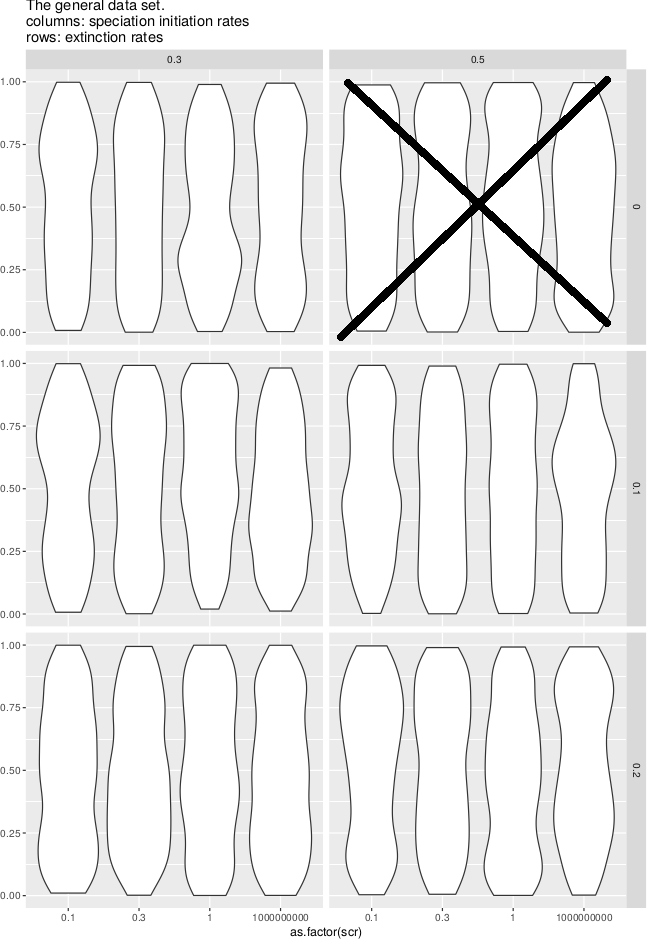
\includegraphics[width=0.8\textwidth]{fig_general.png}
  \caption{
    nLTT statistic distribution per biological parameter set, using the
    balanced data set
  }
\end{figure}

\begin{figure}[!htbp]
  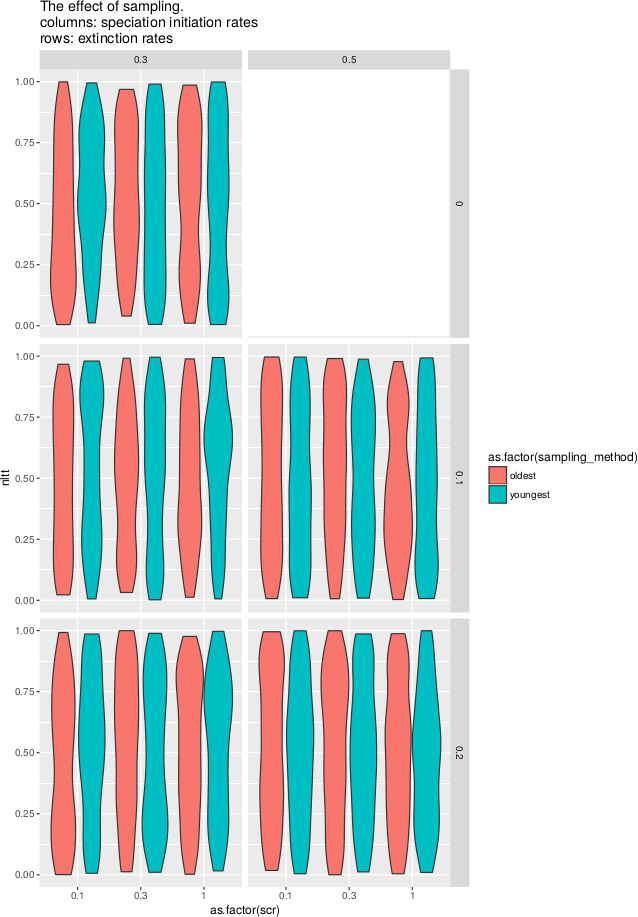
\includegraphics[width=0.8\textwidth]{fig_sampling.png}
  \caption{
    nLTT statistic distribution per biological parameter set per sampling
    regime, using the data set conditioned on sampling regime having an effect 
  }
\end{figure}

%%%%%%%%%%%%%%%%%%%%%%%%%%%%%%%%%%%%%%%%%%%%%%%%%%%%%%%%%%%%%%%%%%%%%%%%%%%%%%%%%%%%%%
\section{Glossary}
%%%%%%%%%%%%%%%%%%%%%%%%%%%%%%%%%%%%%%%%%%%%%%%%%%%%%%%%%%%%%%%%%%%%%%%%%%%%%%%%%%%%%%
% Please supply, as a separate list, the definitions of field-specific terms used in your article.
%%%%%%%%%%%%%%%%%%%%%%%%%%%%%%%%%%%%%%%%%%%%%%%%%%%%%%%%%%%%%%%%%%%%%%%%%%%%%%%%
\begin{table}
  \centering 
  \begin{tabular}{l p{0.6\textwidth}}
    \hline
    Term                  & Definition \\
    \hline
    \hline
    Phylogenetics         & The inference of evolutionary relationships of groups of organisms using genetics \\
    Model prior           & Knowledge or assumptions about the ontogeny of evolutionary histories \\
    Posterior             & A collection of phylogenies and parameter estimates, in which more probable combinations (determined by the data and the model prior) are presented more frequently \\
    Protracted speciation & The process in which speciation takes two events to complete: a speciation-initiation event and a speciation-completion event  \\
    Speciation initiation & The start of a speciation event creating an incipient species \\
    Speciation completion & The end of a speciation event, in which an incipient species is recognized as a good species \\
    \hline
  \end{tabular}
  \caption{
    Glossary
  }
  \label{table:glossary}
\end{table}
%%%%%%%%%%%%%%%%%%%%%%%%%%%%%%%%%%%%%%%%%%%%%%%%%%%%%%%%%%%%%%%%%%%%%%%%%%%%%%%%


%%%%%%%%%%%%%%%%%%%%%%%%%%%%%%%%%%%%%%%%%%%%%%%%%%%%%%%%%%%%%%%%%%%%%%%%%%%%%%%%%%%%%%
%\section{Acknowledgements}
%%%%%%%%%%%%%%%%%%%%%%%%%%%%%%%%%%%%%%%%%%%%%%%%%%%%%%%%%%%%%%%%%%%%%%%%%%%%%%%%%%%%%%

%\textbf{[NOTE: journal does not request for this. Suggest to remove, but how to acknowledge Peregrine otherwise?]}
%We would like to thank the Center for Information Technology of the University of Groningen for their support
%and for providing access to the Peregrine high performance computing cluster.

%%%%%%%%%%%%%%%%%%%%%%%%%%%%%%%%%%%%%%%%%%%%%%%%%%%%%%%%%%%%%%%%%%%%%%%%%%%%%%%%%%%%%%
%\section{Authors' contributions}
%%%%%%%%%%%%%%%%%%%%%%%%%%%%%%%%%%%%%%%%%%%%%%%%%%%%%%%%%%%%%%%%%%%%%%%%%%%%%%%%%%%%%%

%\textbf{[NOTE: journal does not request for this]}
%RSE conceived the idea for this experiment. 
%RJCB created and tested the experiment, 
%and wrote the first draft of the manuscript. 
%RSE contributed substantially to revisions.

% Bibliography
%%%%%%%%%%%%%%%%%%%%%%%%%%%%%%%%%%%%%%%%%%%%%%%%%%%%%%%%%%%%%%%%%%%%%%%%%%%%%%%%%%%%%%
% MEE style
\bibliographystyle{mee}
\bibliography{article}
%%%%%%%%%%%%%%%%%%%%%%%%%%%%%%%%%%%%%%%%%%%%%%%%%%%%%%%%%%%%%%%%%%%%%%%%%%%%%%%%%%%%%%

%%%%%%%%%%%%%%%%%%%%%%%%%%%%%%%%%%%%%%%%%%%%%%%%%%%%%%%%%%%%%%%%%%%%%%%%%%%%%%%%%%%%%%
\appendix
%%%%%%%%%%%%%%%%%%%%%%%%%%%%%%%%%%%%%%%%%%%%%%%%%%%%%%%%%%%%%%%%%%%%%%%%%%%%%%%%%%%%%%

%%%%%%%%%%%%%%%%%%%%%%%%%%%%%%%%%%%%%%%%%%%%%%%%%%%%%%%%%%%%%%%%%%%%%%%%%%%%%%%%
\begin{table}
  \centering 
  \begin{tabular}{l l l}
    \hline
    Parameter             & Description & Values \\
    \hline
    \hline
    $b_g$                 & Speciation initiation rate of a good species & 0.3, 0.5 \\
    $b_i$                 & Speciation initiation rate of an incipient species & 0.3, 0.5 \\
    $\lambda$             & Speciation completion rate & 0.1, 0.3, 1.0, $\infty$ \\
    $\mu_g$               & Extinction rate of a good species & 0.0, 0.1, 0.2 \\
    $\mu_i$               & Extinction rate of an incipient species & 0.0, 0.1, 0.2, 0.4 \\
    \hline
    $t_c$                 & Crown age & 15 \\
    $\sigma_c$            & Standard deviation around crown age & 0.001 \\
    $M$                   & Sampling method & 'shortest', 'longest' or random \\
    $r$                   & Mutation rate & $\frac{1}{15}$ \\
    $l_a$                 & DNA alignment length & $15K$ \\
    $f_i$                 & MCMC sampling interval & 1K or more \\
    $R_i$                 & RNG seed incipient tree and randomly sampled species tree & 1 to 20K \\
    $R_a$                 & RNG seed alignment simulation & $R_i$ \\
    $R_b$                 & RNG seed BEAST2 & $R_i$ \\
    \hline
  \end{tabular}
  \caption{
    Overview of the 12 simulation parameters. Above the horizontal line is 
    the biological parameter set. Sampling method $M$ is random for the general
    data set. For the data set exploring the effect of sampling, we use 'shortest'
    for odd values of $R_i$, and 'longest' for even values of $R_i$.
    $R_i$ is 1 for the first simulation, 2 for the next, etcetera.
  }
  \label{table:parameters}
\end{table}
%%%%%%%%%%%%%%%%%%%%%%%%%%%%%%%%%%%%%%%%%%%%%%%%%%%%%%%%%%%%%%%%%%%%%%%%%%%%%%%%

%%%%%%%%%%%%%%%%%%%%%%%%%%%%%%%%%%%%%%%%%%%%%%%%%%%%%%%%%%%%%%%%%%%%%%%%%%%%%%%%
\begin{table}
  \centering 
  \begin{tabular}{l l}
    \hline
    $n$ & Description \\
    \hline
    \hline
    $12$   & simulation parameters, see table \ref{table:parameters} \\
    $1000$ & nLTT statistic values \\
    $11$ & ESSes of all parameters estimated by BEAST2 (see specs below) \\
    \hline
  \end{tabular}
  \caption{
    Specification of the data sets. Each row will contain one experiment,
    where the columns contain parameters, measurements and diagnostics.
    This table displays the content of the columns. 
    $n$ denotes the number
    of columns a certain item will occupy, resulting in a table of 
    1023 columns and 20K rows.
  }
  \label{table:specs}
\end{table}
%%%%%%%%%%%%%%%%%%%%%%%%%%%%%%%%%%%%%%%%%%%%%%%%%%%%%%%%%%%%%%%%%%%%%%%%%%%%%%%%

%%%%%%%%%%%%%%%%%%%%%%%%%%%%%%%%%%%%%%%%%%%%%%%%%%%%%%%%%%%%%%%%%%%%%%%%%%%%%%%%
\begin{table}
  \centering 
  \begin{tabular}{l l}
    \hline
    \# & Description \\
    \hline
    \hline
    1 & posterior \\
    2 & likelihood \\
    3 & prior \\
    4 & treeLikelihood \\
    5 & TreeHeight \\
    6 & BirthDeath \\
    7 & BDBirthRate \\
    8 & BDDeathRate \\
    9 & logP.mrca \\
    10 & mrcatime \\
    11 & clockRate \\
    \hline
  \end{tabular}
  \caption{
    Overview of the 11 BEAST2 estimated parameters
  }
  \label{table:estimated_parameters}
\end{table}
%%%%%%%%%%%%%%%%%%%%%%%%%%%%%%%%%%%%%%%%%%%%%%%%%%%%%%%%%%%%%%%%%%%%%%%%%%%%%%%%


\end{document}
